Al fine di progettare un'applicazione usabile è utile ottenere informazioni su applicazioni
esistenti, in modo da poter effettuare comparazioni utili. Si è perciò effettuato un discount usability
test con utenti reali su applicazioni concorrenti, scegliendo una base d'utenza con una distribuzione simile
a quella riscontrata durante l'analisi etnografica. Si sono inoltre selezionate applicazioni mobili molto diffuse.
Procediamo quindi all'esposizione dei dettagli emersi durante la valutazione delle applicazioni esistenti.

\subsection{Metodologia di test}
La valutazione delle applicazioni esistenti è stata effettuata secondo due
modalità: un \emph{expert usability review} da noi effettuata e un
\emph{discount usability test}.  Rispetto a quest'ultimo si è utilizzata la
metodologia \emph{thinking aloud}, nella quale gli utenti sono stati invitati a
compiere svariati task descrivendo l'azione intrapresa.  Una volta completato il
task è stato richiesto ai partecipanti di dare una valutazione all'immediatezza
del compito utilizzando una scala Likert con valori compresi fra 1 (per niente
intuitivo) e 5 (immediato).  Nel caso in cui il task sia risultato impossibile
si è attribuito alla facilità di completamento il valore 0.
\subsubsection{Linee guida}
Per valutare l'usabilità delle applicazioni in esame si sono dapprima considerate le
funzionalità principali tramite expert usability review.  In questa fase si è
cercato di esaminare la facilità di navigazione, la completezza funzionale
dell'applicazione e alcune funzioni legate all'accessibilità. 
Oltre ad una descrizione informale dei punti di forza e delle debolezze delle applicazioni in esame,
si è poi proceduto a valutare (in fig. \ref{fig:valutazionelineeguida}) la facilità di navigazione, la ricchezza
di contenuti, la presenza di funzionalità social e la facilità di scoperta di nuove ricette nelle app.
A tal fine si è utilizzata una scala compresa fra 1 e 5, dove 1 indica un punto di debolezza, mentre
5 indica un aspetto ben implementato.\\
\begin{figure}[H]
 \centering
 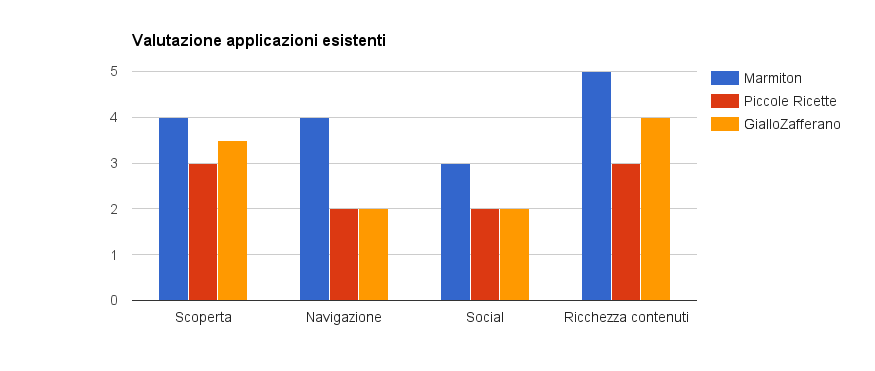
\includegraphics[width=\textwidth]{img/valutazionelineeguida}
 \label{fig:valutazionelineeguida}
\end{figure}
Durante la fase
di \emph{user testing} si è privilegiata invece un'analisi focalizzata su task
fondamentali del dominio in esame.  In questa maniera è possibile ottenere
indicazioni sull'utilizzo ordinario delle applicazioni e sulle loro
funzionalità.  L'unica eccezione a questo approccio riguarda una funzionalità di
accessibilità quale la possibilità di modificare la dimensione del testo.\\
Si riporta in seguito la lista dei task selezionati:
\begin{enumerate}
	\item Cercare una ricetta da noi precedentemente individuata;
	\item Aggiungere una ricetta ai preferiti;
	\item Aggiungere gli ingredienti di una ricetta alla lista della spesa;
	\item Cercare ricette appartenenti ad una determinata categoria
		(vegetariane);
	\item Condividere una ricetta tramite social network;
	\item Creare un menù per la cena o per il pranzo, composto da tre portate;
	\item Cercare istruzioni video relative ad una ricetta;
	\item Cercare commenti relativi ad una ricetta;
	\item Inserire un commento personale riguardo ad una ricetta;
	\item Effettuare la spesa, spuntando uno ad uno gli alimenti;
	\item Cercare un abbinamento per una ricetta specifica;
	\item Cercare ricette nuove proposte dall'applicazione;
	\item Cambiare la dimensione del testo.
\end{enumerate}

\subsection{Applicazioni utilizzate per il test comparativo}
Sono state selezionate tre applicazioni mobili disponibili sui principali sistemi operativi mobili
e testate utilizzando il sistema operativo Android.  Si riporta la lista delle
suddette applicazioni:
\begin{itemize}
	\item Piccole ricette\cite{PiccoleRicette}, piccola applicazione avente una base d'utenza
	limitata e un numero rilevante di ricette (circa 1800).
\item GialloZafferano\cite{GialloZafferano}, applicazione mobile dai gestori dell'omonimo
	sito, popolare e con base di ricette notevole (circa 3400).
\item Marmiton\cite{Marmiton}, applicazione francese con una grande base d'utenza e
	un massiccio numero di ricette disponibili (circa 64.000).
\end{itemize}

\subsection{Piccole Ricette}
È stata utilizzata la versione gratuita del programma, contenente pubblicità
all'avvio in forma di video, che risulta essere molto intrusiva.  La navigazione
dell'applicazione non è immediata, in quanto ad esempio il menù laterale viene
utilizzato soltanto per accedere alle impostazioni e viola concetti fondamentali
di usabilità quali coerenza esterna. Infatti, solitamente,
i menù laterali vengono utilizzati dalle applicazioni come menù di navigazione.
La lista della spesa non presenta checkbox e non rende chiara la modalità di interazione 
con i vari elementi, non presentando inviti o aiuti per gli utenti. La ricerca
risulta essere invece molto espressiva. Nei risultati della ricerca, le
ricette sono descritte tramite simboli, il cui significato non è chiaro.
Non viene espresso in modo chiaro il senso di progressione tra i vari passi della ricetta.

\subsection{GialloZafferano}
Anche in questo caso è stata utilizzata la versione gratuita dell'applicazione.
Quest'ultima, per effettuare operazioni sulle singole ricette, utilizza un menù
contestuale, attivato dal simbolo ``+'' e contenente un semicerchio di icone.
Queste ultime, oltre ad essere numerose, risultano poco chiare, non fornendo legenda o descrizione
testuale.  Per quanto riguarda le
istruzioni in forma di video, una volta avviata la riproduzione, risulta complesso interromperla e essa prosegue
anche quando il video non è più in primo piano.
È presente una modalità per la condivisione tramite mail che non
risulta però essere di facile comprensione ed utilizzo.  L'applicazione non rende chiaro
all'utente il senso di progresso durante la preparazione di una ricetta.
Riguardo all'accessibilità, l'applicazione presenta un'impostazione per
modificare la dimensione del testo, la quale utilizza uno slider il cui
indicatore è colorato come lo sfondo.
Questo rende complicato individuare quale sia l'interazione possibile con tale widget.

\subsection{Marmiton}
Nonostante si tratti di un'applicazione in lingua francese, sia dall'expert
usability review, sia negli user test presentati in seguito, Marmiton è
risultata essere l'applicazione più apprezzata.  Essa è ricca di funzionalità e
contiene il database di ricette più esteso fra quelli considerati.  Permette
inoltre diverse modalità di scoperta delle ricette, proponendo
selezioni tematiche (es. ricette natalizie, grandi classici, ricette del giorno)
e un'interessante modalità per ottenere una ricetta casuale scuotendo il telefono.
La principale critica che è possibile muovere a tale
applicazione riguarda il menù laterale, che risulta leggermente prolisso. Un
altro problema riguarda la separazione tra video e le ricette stesse: nella
pagina relativa alle istruzioni di cucina vengono infatti presentati video correlati, che
non sono relativi alla ricetta in esame. Tale discrepanza potrebbe essere fonte di confusione.
L'applicazione, infine, presenta le migliori funzionalità sociali, permettendo di
condividere le foto delle ricette appena preparate e
di sapere quante persone hanno aggiunto una ricetta ai propri
preferiti.



\subsection{Task e risultati dei test}
Si riportano quindi le soddisfazioni indicate dagli utenti
per i task descritti in precedenza, in relazione ad ogni applicazione in esame:

\subsubsection{Cercare una ricetta}
È stata selezionata una ricetta d'esempio per ogni applicazione, il task è stato
mediamente svolto senza problemi.  A volte non è stata compresa appieno
l'interfaccia di navigazione di ``Piccole ricette''.\\\\
\begin{tabular}{l c}
Piccole Ricette: & 3,5\\
GialloZafferano: & 4,5\\
Marmiton: & 4,3\\
\end{tabular}

\subsubsection{Aggiungere una ricetta ai preferiti}
Viene mantenuta la ricetta precedente.  Sempre per l'applicazione ``Piccole
ricette'' sussiste qualche problema nella comprensione delle funzioni associate ai
simboli ``stellina'' e ``cuoricino''.\\\\
\begin{tabular}{l c}
Piccole Ricette: & 2,8\\
GialloZafferano: & 3,3\\
Marmiton: & 4,1\\
\end{tabular}

\subsubsection{Aggiungere una ricetta alla lista della spesa}
Non sono stati segnalati particolari problemi durante l'esecuzione del
task.\\\\
\begin{tabular}{l c}
Piccole Ricette: & 3,3\\
GialloZafferano: & 3\\
Marmiton: & 4,4\\
\end{tabular}

\subsubsection{Cercare ricette che non presentino uno specifico ingrediente o di
una determinata classe}
In questo caso l'interazione non è chiara, per alcune applicazione viene
utilizzata la ricerca con testo libero, per ``Piccole ricette'' viene utilizzata la
ricerca avanzata.  Il task in ogni caso viene completato correttamente da tutti
i partecipanti.\\\\
\begin{tabular}{l c}
Piccole Ricette: & 3\\
GialloZafferano: & 3,3\\
Marmiton: & 2,7\\
\end{tabular}

\subsubsection{Condividere una ricetta}
Non sono stati rilevati evidenti problemi di usabilità legati al task in
esame.  Le ricette sono state condivise sui principali social network o tramite
sistemi di instant messaging.\\\\
\begin{tabular}{l c}
Piccole Ricette: & 4,3\\
GialloZafferano: & 4\\
Marmiton: & 4,3\\
\end{tabular}

\subsubsection{Creare un menù}
Il task viene mediamente risolto, in alcuni casi l'utente è risultato abbastanza
confuso da funzionalità relative ai menù poco evidenti. Tali funzione causano spesso fra gli utenti confusione tra lista
della spesa e creazione di menù tematici.\\\\
\begin{tabular}{l c}
Piccole Ricette: & 3,5\\
GialloZafferano: & 2,6\\
Marmiton: & 3,7\\
\end{tabular}

\subsubsection{Cercare istruzioni video}
Come già rilevato nella fase precedente ``Marmiton'' presenta qualche problema legato
alle istruzioni video, che risultano scomode e non di facile reperibilità. Anche
``GialloZafferano'' soffre degli stessi problemi, risultando di difficile utilizzo.\\\\
\begin{tabular}{l c}
Piccole Ricette: & 3,2\\
GialloZafferano: & 2,8\\
Marmiton: & 2,6\\
\end{tabular}

\subsubsection{Cercare commenti}
Il compito viene completato in brevissimi tempi e con grande facilità da parte
della totalità dei partecipanti.\\\\
\begin{tabular}{l c}
Piccole Ricette: & 4,5\\
GialloZafferano: & 5\\
Marmiton: & 4,3\\
\end{tabular}

\subsubsection{Inserire un commento personale}
Anche in questo caso il compito è stato completato egregiamente da ogni
utente.\\\\
\begin{tabular}{l c}
Piccole Ricette: & 4,6\\
GialloZafferano: & 4,3\\
Marmiton: & 4,3\\
\end{tabular}

\subsubsection{Effettuare la spesa}
Il task non è risultato problematico.  Qualche piccola difficoltà è emersa nella navigazione
dell'applicazione ``GialloZafferano'', dovuta alle problematiche suddette del menù ``+''.
Lievemente problematica risulta anche l'interazione con gli ingredienti in ``Piccole
ricette''.\\\\
\begin{tabular}{l c}
Piccole Ricette: & 4\\
GialloZafferano: & 3\\
Marmiton: & 3,6\\
\end{tabular}

\subsubsection{Cercare abbinamenti suggeriti}
Nelle applicazioni la ricerca di abbinamenti risulta spesso difficoltosa, causando
un abbandono del task da parte degli utenti. 
Al fine di completare il compito i partecipanti hanno spesso utilizzato i commenti o
il testo di descrizione della ricetta.\\\\
\begin{tabular}{l c}
Piccole Ricette: & 0\\
GialloZafferano: & 0,5\\
Marmiton: & 1,3\\
\end{tabular}

\subsubsection{Cercare ricette nuove proposte dall'applicazione stessa}
Il task risulta semplice, data anche la numerosa presenza di ricette tematiche
per l'imminente festività natalizia nel periodo del test.\\\\
\begin{tabular}{l c}
Piccole Ricette: & 3,6\\
GialloZafferano: & 4,5\\
Marmiton: & 4,6\\
\end{tabular}

\subsubsection{Cambiare dimensioni del testo}
Il task è probabilmente il più problematico tra quelli analizzati fin'ora, è spesso impossibile
completarlo e, ove possibile, l'interazione risulta
scomoda e non intuitiva.  Viene quasi sempre tentata
un'interazione di tipo \emph{pinch to zoom} senza successo.\\\\
\begin{tabular}{l c}
Piccole Ricette: & 0\\
GialloZafferano: & 3\\
Marmiton: & 0\\
\end{tabular}
